\documentclass[aspectratio=169, 10pt]{beamer}

\usetheme{CambridgeUS}
\usecolortheme{dolphin}

\usepackage{advdate}
\usepackage{animate}
\usepackage{siunitx}
\usepackage{tikz}

\graphicspath{{./figs_cropped/}}


\title{CPEX-AW Forecast \vspace{-1cm}}
\author{Lead Forecaster, Forecaster 2, Forecaster 3\vspace{-1cm}}
\date{{\AdvanceDate[0]\today}\vspace{-1cm}}
\logo{
\includegraphics[width=1.5cm]{logo_cpexcv.png}}

\begin{document}

\begin{frame}
\vspace{-3cm}
\titlepage

\vspace{-.2cm}
\textbf{Current \\conditions:}

\vspace{.5cm}
\textbf{Day 1:}

\vspace{.5cm}
\textbf{Day 2:}

\vspace{.5cm}
\textbf{Outlook \\(days 3-5):}

\vspace{-1.5cm}
\end{frame}

%%%%%%%%%%%%%%%%%%%%%%%%%%%%%%%%%
%%%%%%%%%%%%%%%%%%%%%%%%%%%%%%%%%
%%%%%%%%%%%%%%%%%%%%%%%%%%%%%%%%%
% % % % % Current conditions - synoptic view
\begin{frame}
\vspace{-1cm}
\frametitle{Current conditions - synoptic view}

\begin{figure} [htbp]
\begin{center}
\vspace{.6cm}
\textbf{NHC Surface Analysis}

\frame{\IfFileExists{./figs_cropped/NHC_surface_analysis.png}{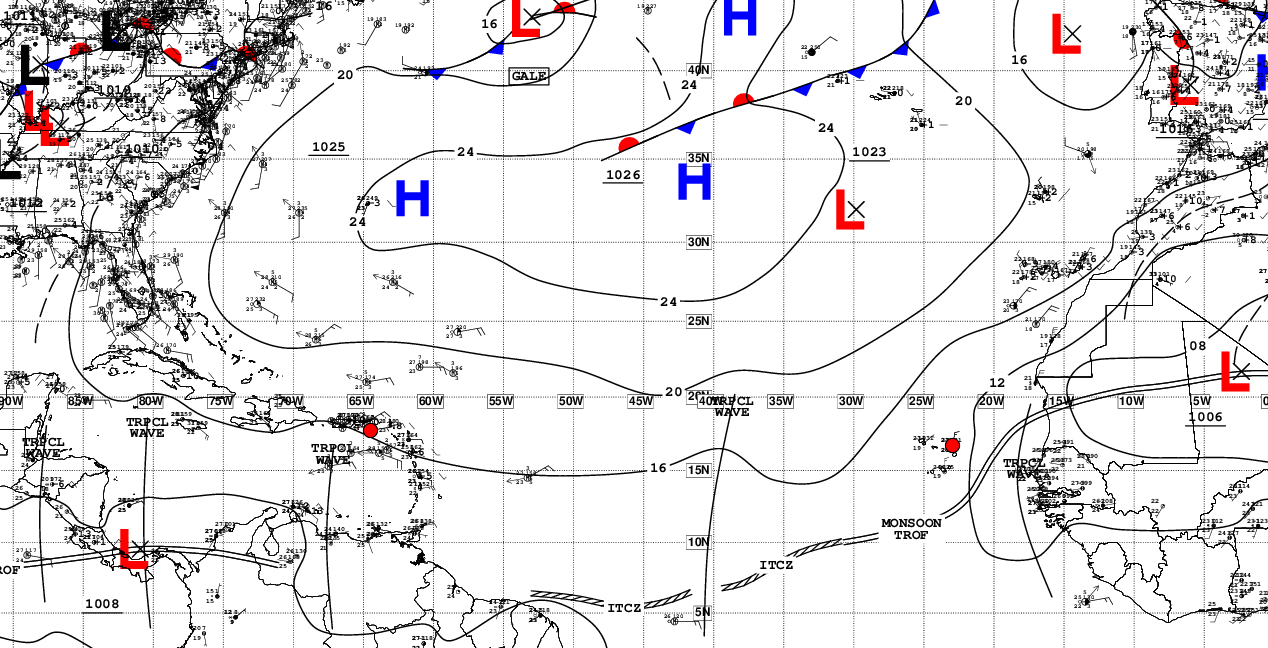
\includegraphics[height=.75\textheight]{NHC_surface_analysis.png}}{
\includegraphics[height=.75\textheight]{logo_cpexcv.png}}}
\end{center}
\end{figure}

\end{frame}





%%%%%%%%%%%%%%%%%%%%%%%%%%%%%%%%%
%%%%%%%%%%%%%%%%%%%%%%%%%%%%%%%%%
%%%%%%%%%%%%%%%%%%%%%%%%%%%%%%%%%
% % % % % Current conditions - ITCZ and AEW (African Easterly Waves)
\begin{frame}
\frametitle{Current conditions - ITCZ and AEW}
\begin{columns}
\begin{column}{0.47\textwidth}
\vspace{-.5cm}
\begin{figure}
\textbf{Total Precipitable Water} \\
\frame{\IfFileExists{./figs_cropped/MIMIC-TPW_latest.png}{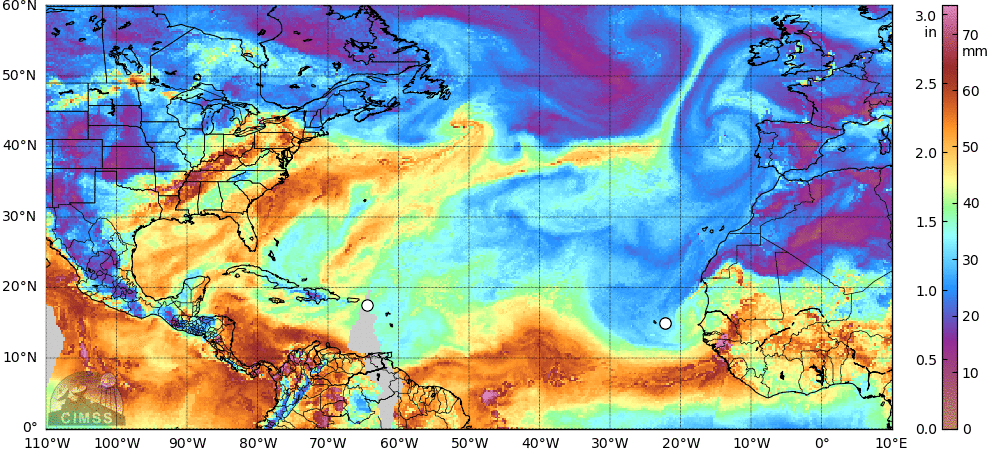
\includegraphics[width=\textwidth]{MIMIC-TPW_latest.png}}{
\includegraphics[height=.25\textheight]{logo_cpexcv.png}}}
\end{figure}
\vspace{-.6cm}
\begin{figure}
\textbf{Model TPW + Clouds} \vspace{.04cm} \\
\frame{\IfFileExists{./figs_cropped/uwincm_clouds_current.jpg}{\includegraphics[height=.38\textheight]{uwincm_clouds_current.jpg}}{
\includegraphics[height=.25\textheight]{logo_cpexcv.png}}}
\end{figure}
\end{column}



\begin{column}{0.53\textwidth}
\vspace{-.47cm}
\begin{figure}
\textbf{IMERG precip, GFS MSLP \& 700 mb $\psi$}\\
\frame{\IfFileExists{./figs_cropped/AEW_Brammer.jpg}{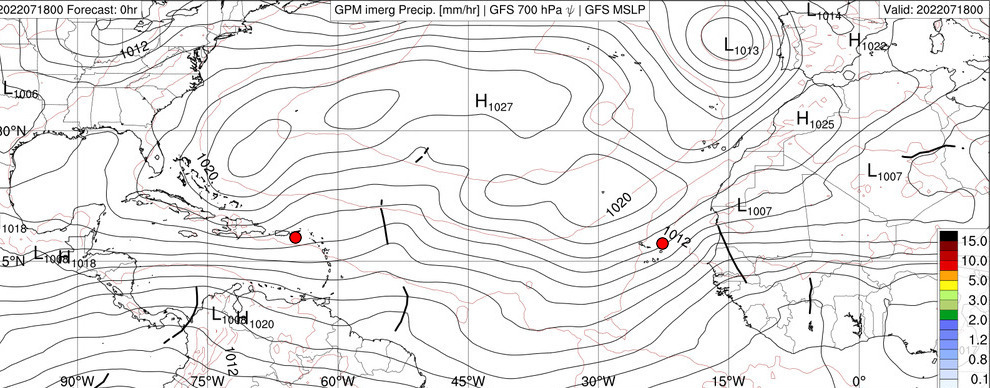
\includegraphics[width=\textwidth]{AEW_Brammer.jpg}}{
\includegraphics[height=.25\textheight]{logo_cpexcv.png}}}
\end{figure}
\vspace{-.15cm}
\begin{figure}
\vspace{-.45cm} \textbf{GOES16 \& Meteosat-11 IR}  \vspace{.1cm}\\
\frame{\IfFileExists{./figs_cropped/Goes16_Meteosat11_IRC.png}{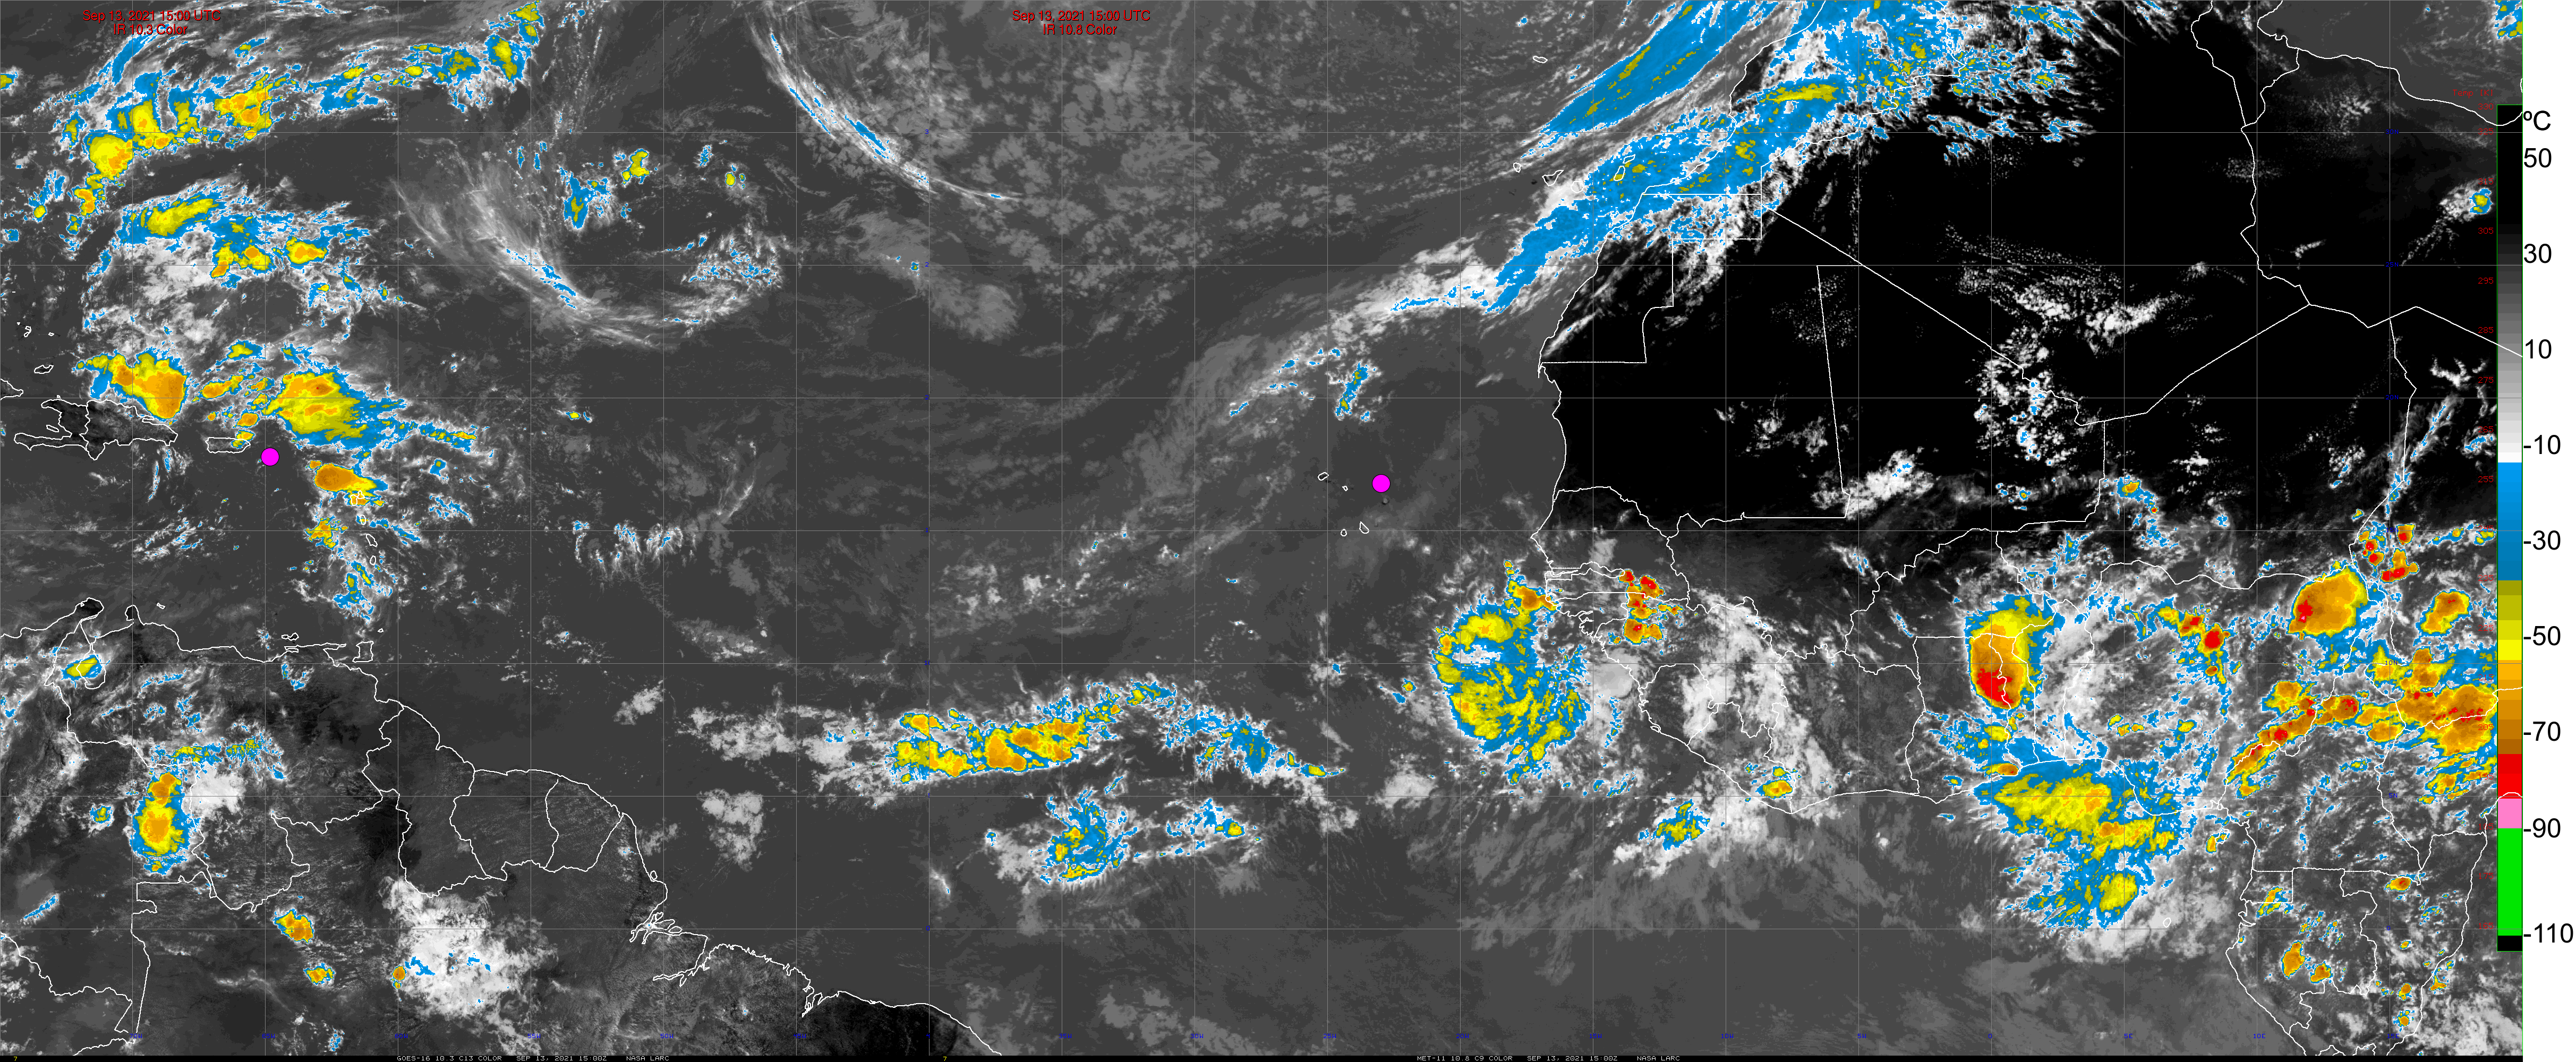
\includegraphics[height=.38\textheight]{Goes16_Meteosat11_IRC.png}}{
\includegraphics[height=.25\textheight]{logo_cpexcv.png}}}
\end{figure}
\end{column}
\end{columns}
\end{frame}

%%%%%%%%%%%%%%%%%%%%%%%%%%%%%%%%%
%%%%%%%%%%%%%%%%%%%%%%%%%%%%%%%%%
%%%%%%%%%%%%%%%%%%%%%%%%%%%%%%%%%
% % % % % Current conditions - Dust and Aerosols
\begin{frame}
\frametitle{Current conditions - dust and aerosols}

\begin{columns}
\begin{column}{0.5\textwidth}


\vspace{-1.4cm}
\begin{figure}
\textbf{Dust and Dry Air} \\
\frame{\IfFileExists{./figs_cropped/SAL_dryAir_split.jpg}{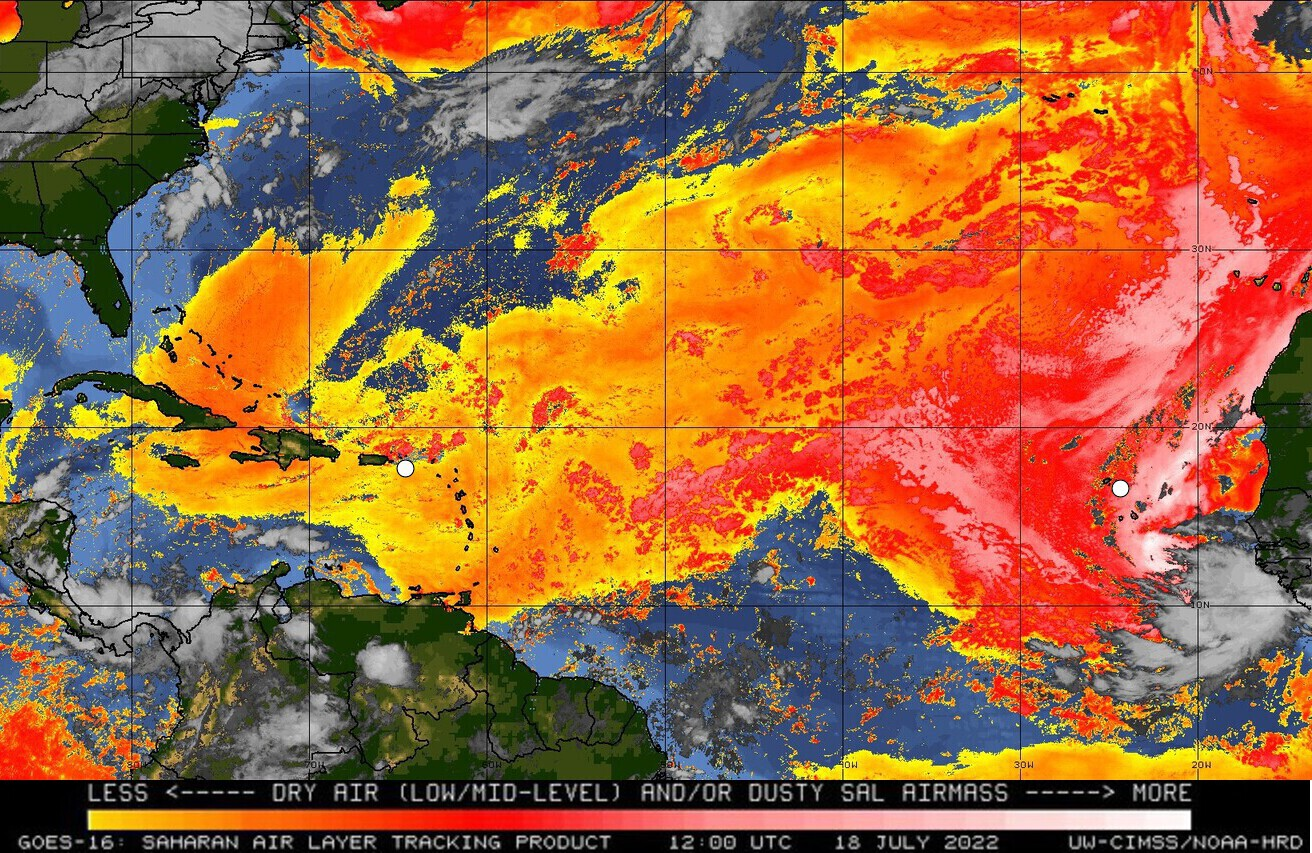
\includegraphics[width=\textwidth]{SAL_dryAir_split.jpg}}{
\includegraphics[height=.25\textheight]{logo_cpexcv.png}}}
\end{figure}

\end{column}
\begin{column}{0.5\textwidth}

\vspace{-1.4cm}
\begin{figure}
\textbf{Dust Aerosol Optical Thickness} \\
\frame{\IfFileExists{./figs_cropped/GEOS_dust_aot.png}{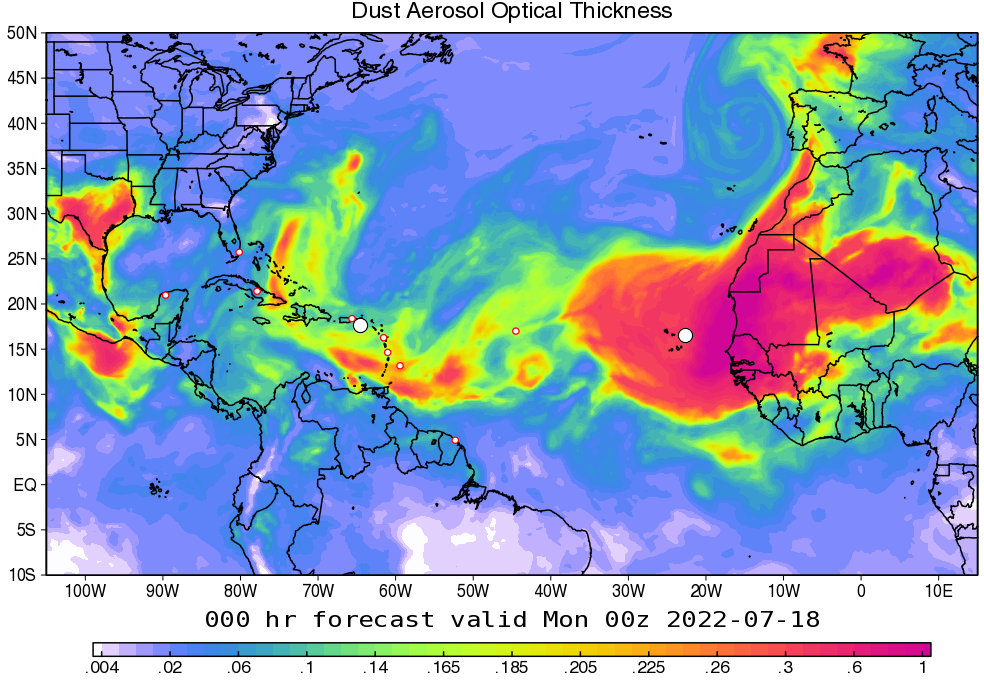
\includegraphics[width=.94\textwidth]{GEOS_dust_aot.png}}{
\includegraphics[height=.25\textheight]{logo_cpexcv.png}}}
\end{figure}

\end{column}
\end{columns}
\vspace{.2cm}
Comments:

\end{frame}

%%%%%%%%%%%%%%%%%%%%%%%%%%%%%%%%%
%%%%%%%%%%%%%%%%%%%%%%%%%%%%%%%%%
%%%%%%%%%%%%%%%%%%%%%%%%%%%%%%%%%
% % % % % NHC Outlook
\begin{frame}
\vspace{-1cm}
\frametitle{NHC Outlook: days 2 \& 5 ({\AdvanceDate[+2]\today}, {\AdvanceDate[+5]\today})}

\vspace{-.3cm}
\begin{columns}
\begin{column}{0.5\textwidth}


\begin{figure}
\textbf{2-day Outlook} \\
\frame{\IfFileExists{./figs_cropped/NHC_2day_outlook.png}{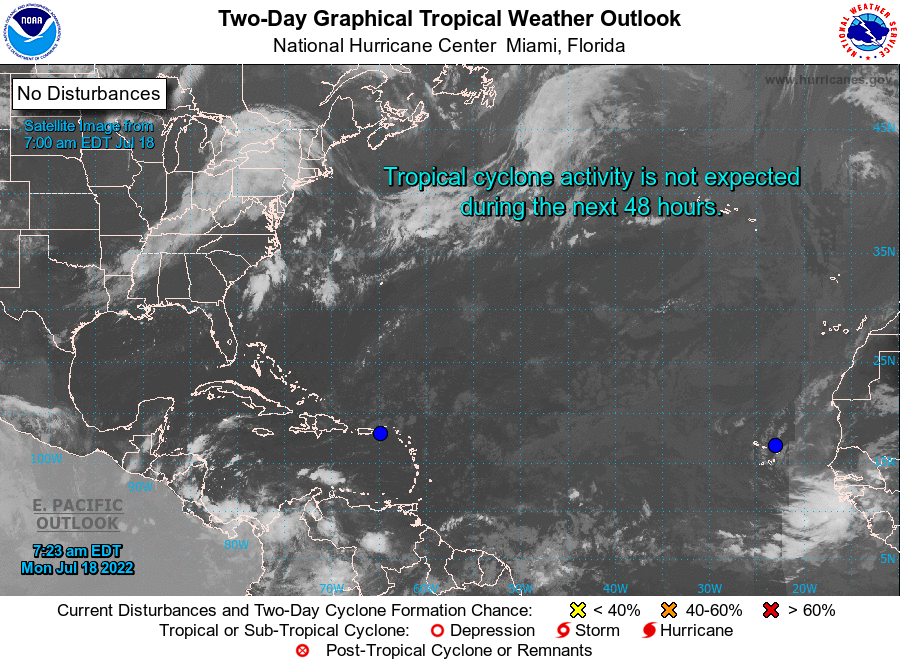
\includegraphics[width=.93\textwidth]{NHC_2day_outlook.png}}{
\includegraphics[height=.25\textheight]{logo_cpexcv.png}}}
\end{figure}

\end{column}
\begin{column}{0.5\textwidth}

\begin{figure}
\textbf{5-day Outlook} \\
\frame{\IfFileExists{./figs_cropped/NHC_5day_outlook.png}{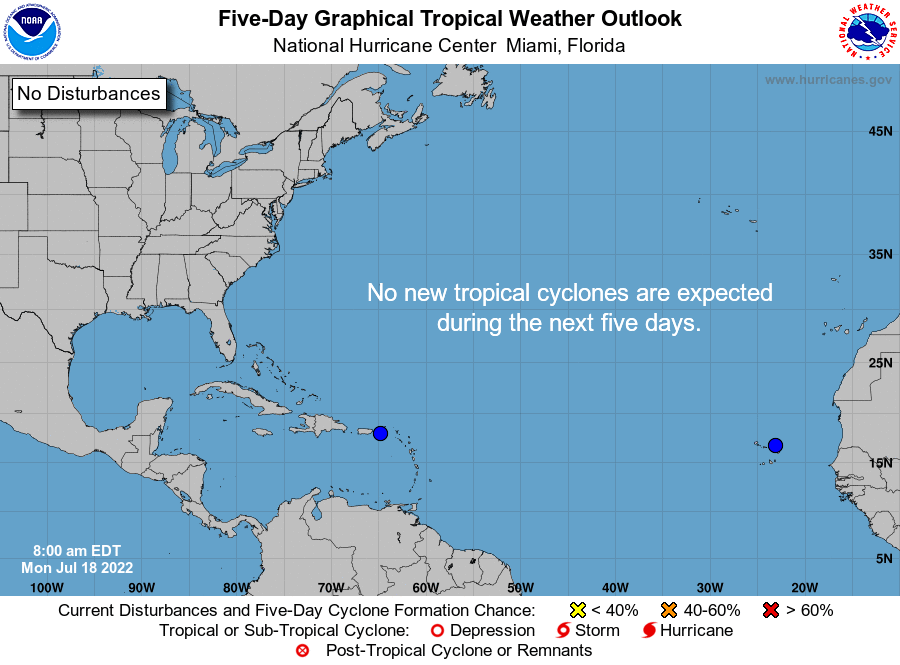
\includegraphics[width=.93\textwidth]{NHC_5day_outlook.png}}{
\includegraphics[height=.25\textheight]{logo_cpexcv.png}}}
\end{figure}

\end{column}
\end{columns}



\end{frame}

%%%%%%%%%%%%%%%%%%%%%%%%%%%%%%%%%
%%%%%%%%%%%%%%%%%%%%%%%%%%%%%%%%%
%%%%%%%%%%%%%%%%%%%%%%%%%%%%%%%%%
% % % % % Day 1 Forecast - slide 1
\begin{frame}
\frametitle{Forecast: day 1 ({\AdvanceDate[+1]\today})}

\vspace{-.2cm}
\begin{columns}
\begin{column}{0.5\textwidth}
\begin{center}
\textbf{Surface Winds}\\
\end{center}
\end{column}

\begin{column}{0.5\textwidth}
\begin{center}
\textbf{650mb RH and Geopotential Height} \\
\end{center}
\end{column}
\end{columns}

\begin{figure}

\frame{\IfFileExists{./figs_cropped/uwincm_joint_surfaceWind_650mbRH_day1_anim_14.jpg}{\animategraphics[autoplay,loop, width=.9\textwidth]{2}{uwincm_joint_surfaceWind_650mbRH_day1_anim_}{00}{14}}{
\includegraphics[height=.25\textheight]{logo_cpexcv.png}}}

\end{figure}


Comments:
\vspace{4cm}


\end{frame}




%%%%%%%%%%%%%%%%%%%%%%%%%%%%%%%%%
%%%%%%%%%%%%%%%%%%%%%%%%%%%%%%%%%
%%%%%%%%%%%%%%%%%%%%%%%%%%%%%%%%%
% % % % % Day 1 Forecast - slide 2
\begin{frame}
\frametitle{Forecast: day 1 ({\AdvanceDate[+1]\today})}

\vspace{-.3cm}
\begin{columns}
\begin{column}{0.5\textwidth}
\begin{center}
\textbf{TPW \& Clouds}\\
\end{center}
\end{column}

\begin{column}{0.5\textwidth}
\begin{center}
\textbf{Boundary Layer Height and Temperature} \\
\end{center}
\end{column}
\end{columns}

\begin{figure}

\frame{\IfFileExists{./figs_cropped/uwincm_joint_clouds_boundaryLayer_day1_anim_14.jpg}{\animategraphics[autoplay,loop, width=.9\textwidth]{2}{uwincm_joint_clouds_boundaryLayer_day1_anim_}{00}{14}}{
\includegraphics[height=.25\textheight]{logo_cpexcv.png}}}
\end{figure}

Comments:
\vspace{4cm}


\end{frame}


%%%%%%%%%%%%%%%%%%%%%%%%%%%%%%%%%
%%%%%%%%%%%%%%%%%%%%%%%%%%%%%%%%%
%%%%%%%%%%%%%%%%%%%%%%%%%%%%%%%%%
% % % % % Day 1 Forecast - slide 3
\begin{frame}
\frametitle{Forecast: day 1 ({\AdvanceDate[+1]\today})}

\vspace{-.3cm}
\begin{columns}
\begin{column}{0.5\textwidth}
\begin{center}
\textbf{Precipitation - UWIN-CM}\\
\end{center}
\end{column}

\begin{column}{0.5\textwidth}
\begin{center}
\textbf{Precipitation - U of Utah} \\
\end{center}
\end{column}
\end{columns}

\begin{figure}


\frame{\IfFileExists{./figs_cropped/uwincm_joint_precip_day1_anim_14.jpg}{\animategraphics[autoplay,loop, width=.9\textwidth]{2}{uwincm_joint_precip_day1_anim_}{00}{14}}{
\includegraphics[height=.25\textheight]{logo_cpexcv.png}}}
\end{figure}

Comments:
\vspace{4cm}


\end{frame}




%%%%%%%%%%%%%%%%%%%%%%%%%%%%%%%%%
%%%%%%%%%%%%%%%%%%%%%%%%%%%%%%%%%
%%%%%%%%%%%%%%%%%%%%%%%%%%%%%%%%%
% % % % % Day 2 Forecast - slide 1
\begin{frame}
\frametitle{Forecast: day 2 ({\AdvanceDate[+2]\today})}

\vspace{-.2cm}
\begin{columns}
\begin{column}{0.5\textwidth}
\begin{center}
\textbf{Surface Winds}\\
\end{center}
\end{column}

\begin{column}{0.5\textwidth}
\begin{center}
\textbf{650mb RH and Geopotential Height} \\
\end{center}
\end{column}
\end{columns}

\begin{figure}

\frame{\IfFileExists{./figs_cropped/uwincm_joint_surfaceWind_650mbRH_day2_anim_14.jpg}{\animategraphics[autoplay,loop, width=.9\textwidth]{2}{uwincm_joint_surfaceWind_650mbRH_day2_anim_}{00}{14}}{
\includegraphics[height=.25\textheight]{logo_cpexcv.png}}}

\end{figure}


Comments:
\vspace{4cm}


\end{frame}




%%%%%%%%%%%%%%%%%%%%%%%%%%%%%%%%%
%%%%%%%%%%%%%%%%%%%%%%%%%%%%%%%%%
%%%%%%%%%%%%%%%%%%%%%%%%%%%%%%%%%
% % % % % Day 2 Forecast - slide 2
\begin{frame}
\frametitle{Forecast: day 2 ({\AdvanceDate[+2]\today})}

\vspace{-.3cm}
\begin{columns}
\begin{column}{0.5\textwidth}
\begin{center}
\textbf{TPW \& Clouds}\\
\end{center}
\end{column}

\begin{column}{0.5\textwidth}
\begin{center}
\textbf{Boundary Layer Height and Temperature} \\
\end{center}
\end{column}
\end{columns}

\begin{figure}

\frame{\IfFileExists{./figs_cropped/uwincm_joint_clouds_boundaryLayer_day2_anim_14.jpg}{\animategraphics[autoplay,loop, width=.9\textwidth]{2}{uwincm_joint_clouds_boundaryLayer_day2_anim_}{00}{14}}{
\includegraphics[height=.25\textheight]{logo_cpexcv.png}}}

\end{figure}

Comments:
\vspace{4cm}


\end{frame}


%%%%%%%%%%%%%%%%%%%%%%%%%%%%%%%%%
%%%%%%%%%%%%%%%%%%%%%%%%%%%%%%%%%
%%%%%%%%%%%%%%%%%%%%%%%%%%%%%%%%%
% % % % % Day 2 Forecast - slide 3
\begin{frame}
\frametitle{Forecast: day 2 ({\AdvanceDate[+2]\today})}

\vspace{-.3cm}
\begin{columns}
\begin{column}{0.5\textwidth}
\begin{center}
\textbf{Precipitation - UWIN-CM}\\
\end{center}
\end{column}

\begin{column}{0.5\textwidth}
\begin{center}
\textbf{Precipitation - U of Utah} \\
\end{center}
\end{column}
\end{columns}

\begin{figure}


\frame{\IfFileExists{./figs_cropped/uwincm_joint_precip_day2_anim_14.jpg}{\animategraphics[autoplay,loop, width=.9\textwidth]{2}{uwincm_joint_precip_day2_anim_}{00}{14}}{
\includegraphics[height=.25\textheight]{logo_cpexcv.png}}}
\end{figure}

Comments:
\vspace{4cm}


\end{frame}





%%%%%%%%%%%%%%%%%%%%%%%%%%%%%%%%%
%%%%%%%%%%%%%%%%%%%%%%%%%%%%%%%%%
%%%%%%%%%%%%%%%%%%%%%%%%%%%%%%%%%
% % % % % Dust and Aerosol forecast - slide 1
\begin{frame}
\frametitle{Forecast: dust and aerosols (current)}

\begin{columns}
\begin{column}{0.33\textwidth}


\vspace{-3.5cm}
\begin{figure}
\textbf{AOT} \vspace{0.0cm}\\
\frame{\IfFileExists{./figs_cropped/GEOS_total_aot.png}{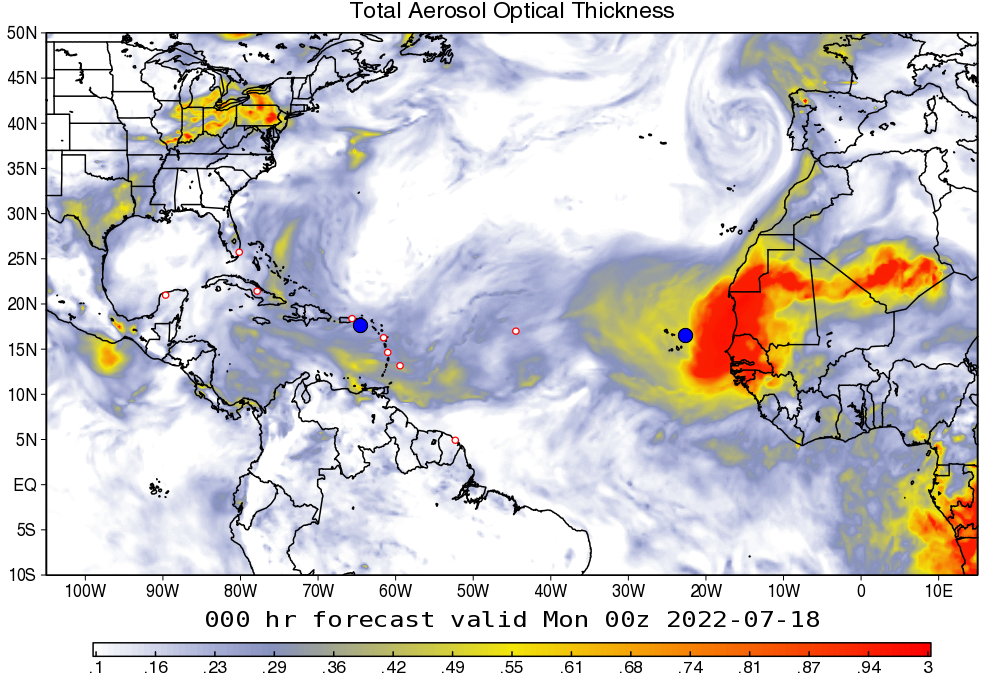
\includegraphics[width=.9\textwidth]{GEOS_total_aot.png}}{
\includegraphics[height=.25\textheight]{logo_cpexcv.png}}}
\end{figure}

\vspace{-.6cm}
\begin{figure}
\textbf{Dust AOT}  \vspace{0.06cm}\\
\begin{tikzpicture}
\node[anchor=south west,inner sep=0] (image) at (0,0) {\frame{\IfFileExists{./figs_cropped/GEOS_dust_aot.png}{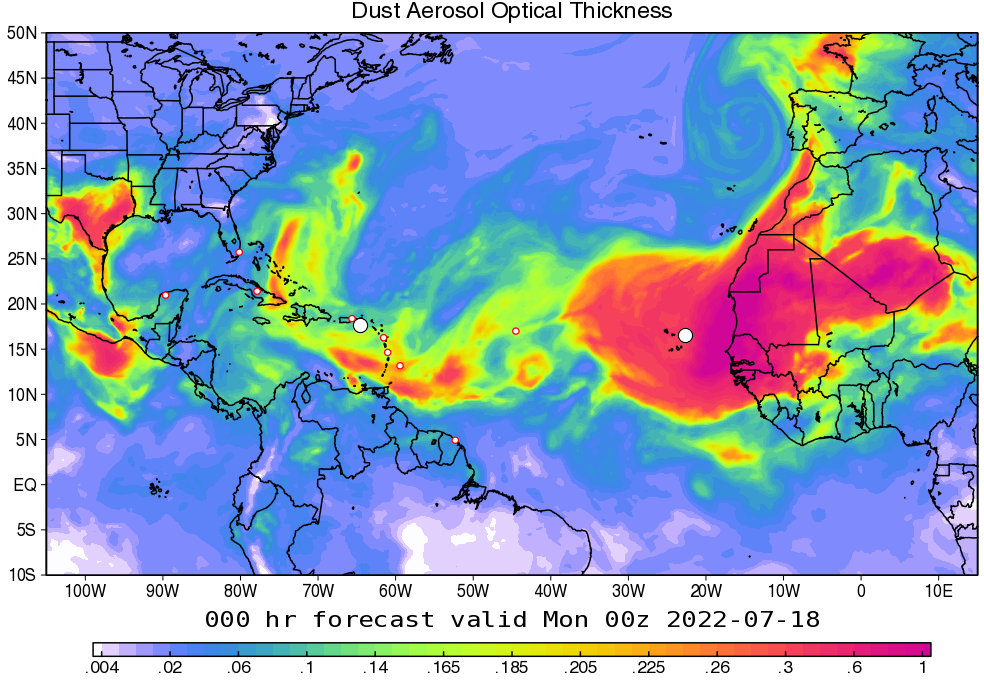
\includegraphics[width=.9\textwidth]{GEOS_dust_aot.png}}{
\includegraphics[height=.25\textheight]{logo_cpexcv.png}}}};
\draw[line width=.2mm, color=black] (1.85,1.) -- (1.85,2.5); %vertical line
\node[text=black] at (1.85, .9) {\tiny 20W};
\draw[line width=.2mm, color=black] (.43,1.6) -- (4., 1.6); %horizontal line
\node[text=black] at (.43, 1.68) {\tiny 15N};
\end{tikzpicture}
\end{figure}
\end{column}

\begin{column}{0.33\textwidth}

\vspace{-0.6cm}
\begin{figure}
\vspace{.1cm}
\textbf{\tiny Cross-section at 15N}  \vspace{0.0cm}\\
\frame{\IfFileExists{./figs_cropped/GEOS_dust_aot_vert_15N.png}{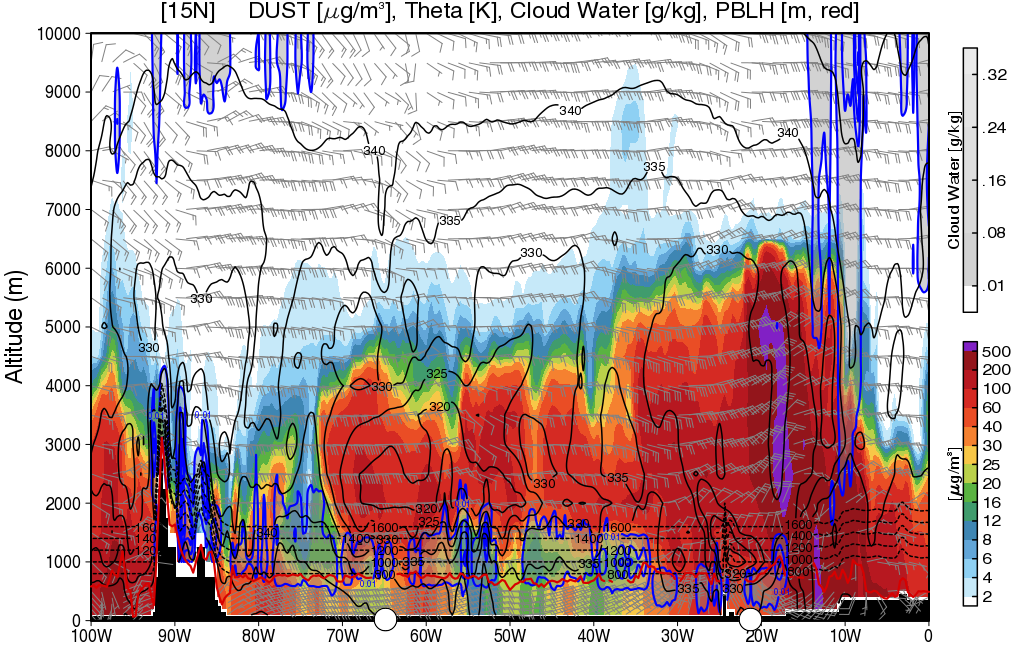
\includegraphics[width=.99\textwidth]{GEOS_dust_aot_vert_15N.png}}{
\includegraphics[height=.25\textheight]{logo_cpexcv.png}}}
\end{figure}


\vspace{-.7cm}
\begin{figure}
\textbf{\tiny Cross-section at 20W}  \vspace{0.0cm}\\
\frame{\IfFileExists{./figs_cropped/GEOS_dust_aot_vert_20W.png}{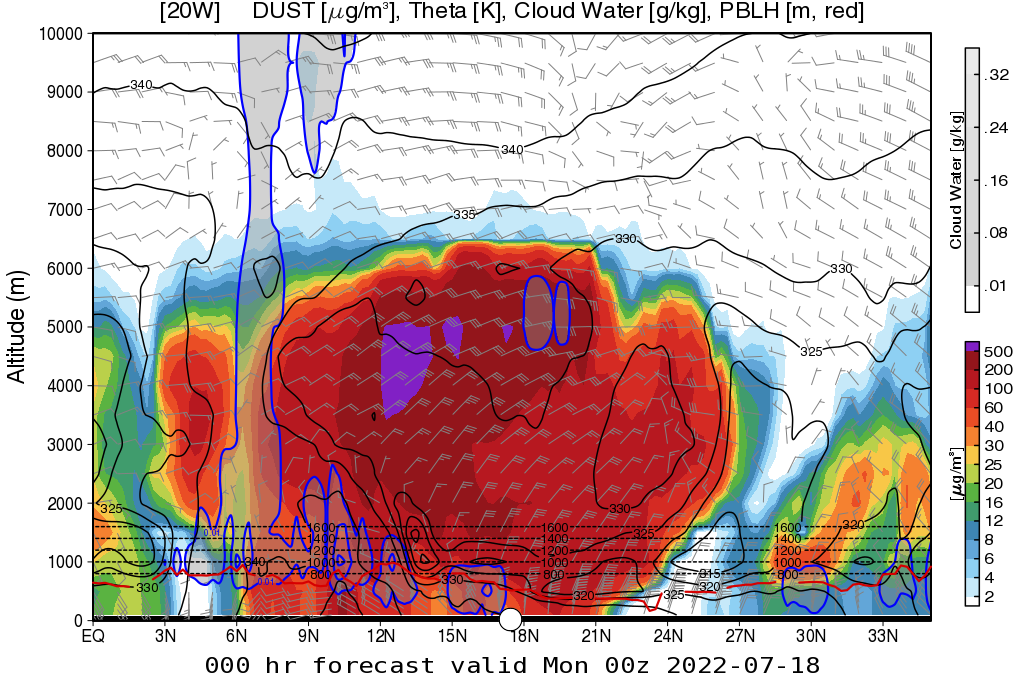
\includegraphics[width=.99\textwidth]{GEOS_dust_aot_vert_20W.png}}{
\includegraphics[height=.25\textheight]{logo_cpexcv.png}}}
\end{figure}

\vspace{2.7cm}


\end{column}

\begin{column}{0.33\textwidth}


\end{column}
\end{columns}

\end{frame}




%%%%%%%%%%%%%%%%%%%%%%%%%%%%%%%%%
%%%%%%%%%%%%%%%%%%%%%%%%%%%%%%%%%
%%%%%%%%%%%%%%%%%%%%%%%%%%%%%%%%%
% % % % % Dust and Aerosol forecast - slide 2
\begin{frame}
\frametitle{Forecast: dust and aerosols (day 1, {\AdvanceDate[+1]\today})}

\begin{columns}
\begin{column}{0.33\textwidth}


\vspace{-3.5cm}
\begin{figure}
\textbf{AOT} \vspace{0.0cm}\\
\frame{\IfFileExists{./figs_cropped/GEOS_total_aot_day1.png}{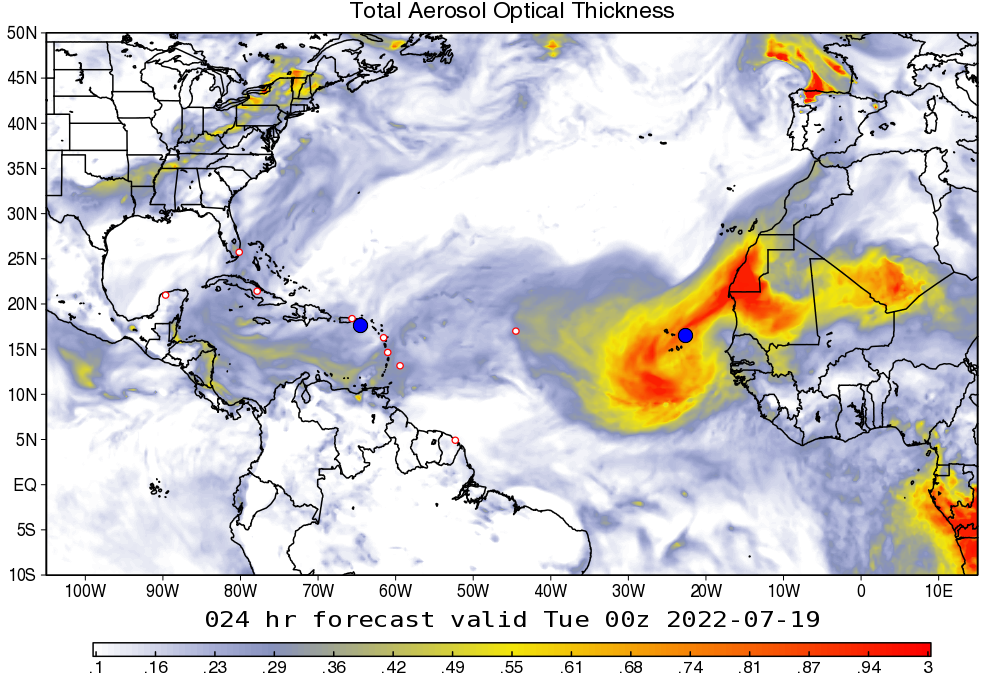
\includegraphics[width=.9\textwidth]{GEOS_total_aot_day1.png}}{
\includegraphics[height=.25\textheight]{logo_cpexcv.png}}}
\end{figure}

\vspace{-.6cm}
\begin{figure}
\textbf{Dust AOT}  \vspace{0.06cm}\\
\begin{tikzpicture}
\node[anchor=south west,inner sep=0] (image) at (0,0) {\frame{\IfFileExists{./figs_cropped/GEOS_dust_aot_day1.png}{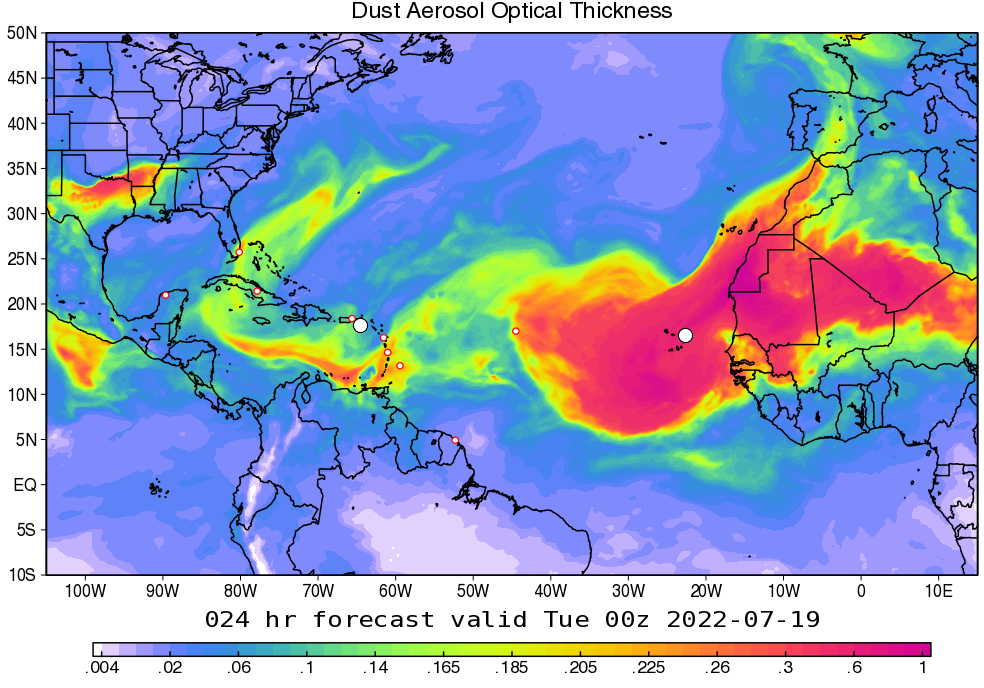
\includegraphics[width=.9\textwidth]{GEOS_dust_aot_day1.png}}{
\includegraphics[height=.25\textheight]{logo_cpexcv.png}}}};
\draw[line width=.2mm, color=black] (1.85,1.) -- (1.85,2.5); %vertical line
\node[text=black] at (1.85, .9) {\tiny 20W};
\draw[line width=.2mm, color=black] (.43,1.6) -- (4., 1.6); %horizontal line
\node[text=black] at (.43, 1.68) {\tiny 15N};
\end{tikzpicture}
\end{figure}
\end{column}


\begin{column}{0.33\textwidth}

\vspace{-0.6cm}
\begin{figure}
\vspace{.1cm}
\textbf{\tiny Cross-section at 15N}  \vspace{0.0cm}\\
\frame{\IfFileExists{./figs_cropped/GEOS_dust_aot_day1_vert_15N.png}{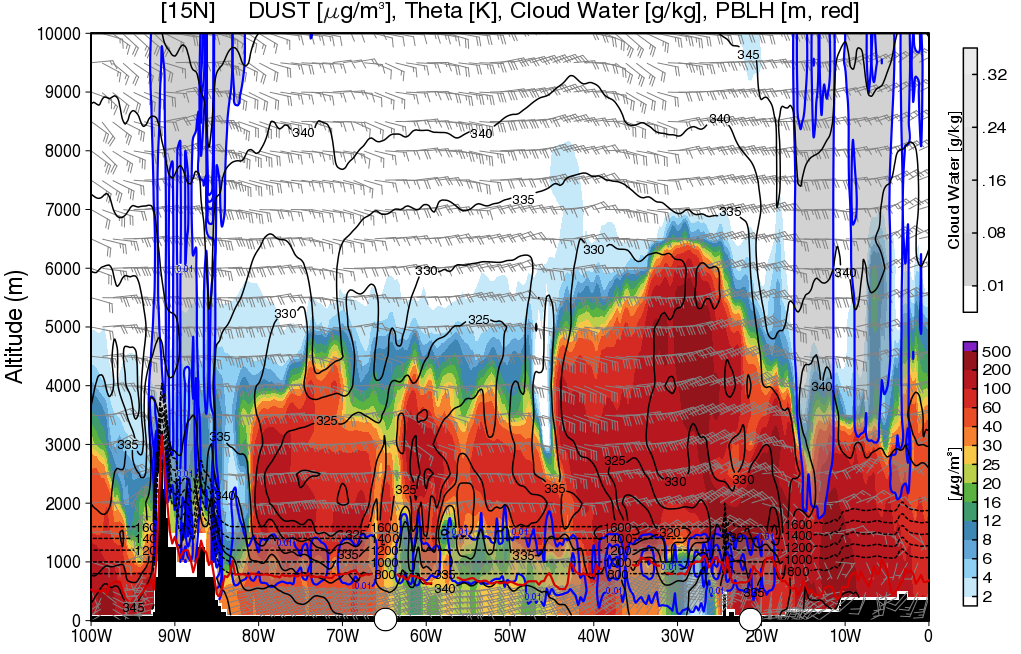
\includegraphics[width=.99\textwidth]{GEOS_dust_aot_day1_vert_15N.png}}{
\includegraphics[height=.25\textheight]{logo_cpexcv.png}}}
\end{figure}


\vspace{-.7cm}
\begin{figure}
\textbf{\tiny Cross-section at 20W}  \vspace{0.0cm}\\
\frame{\IfFileExists{./figs_cropped/GEOS_dust_aot_day1_vert_20W.png}{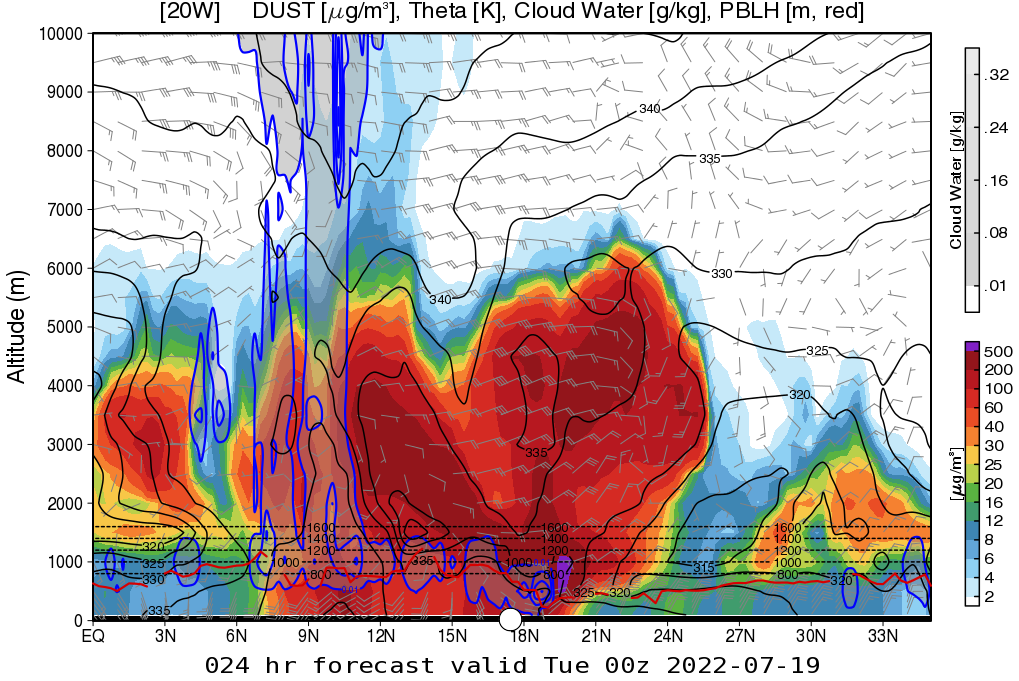
\includegraphics[width=.99\textwidth]{GEOS_dust_aot_day1_vert_20W.png}}{
\includegraphics[height=.25\textheight]{logo_cpexcv.png}}}
\end{figure}

\vspace{2.7cm}


\end{column}

\begin{column}{0.33\textwidth}


\end{column}
\end{columns}

\end{frame}



%%%%%%%%%%%%%%%%%%%%%%%%%%%%%%%%%
%%%%%%%%%%%%%%%%%%%%%%%%%%%%%%%%%
%%%%%%%%%%%%%%%%%%%%%%%%%%%%%%%%%
% % % % % Dust and Aerosol forecast - slide 3
\begin{frame}
\frametitle{Forecast: dust and aerosols (day 2, {\AdvanceDate[+2]\today})}

\begin{columns}
\begin{column}{0.33\textwidth}


\vspace{-3.5cm}
\begin{figure}
\textbf{AOT} \vspace{0.0cm}\\
\frame{\IfFileExists{./figs_cropped/GEOS_total_aot_day2.png}{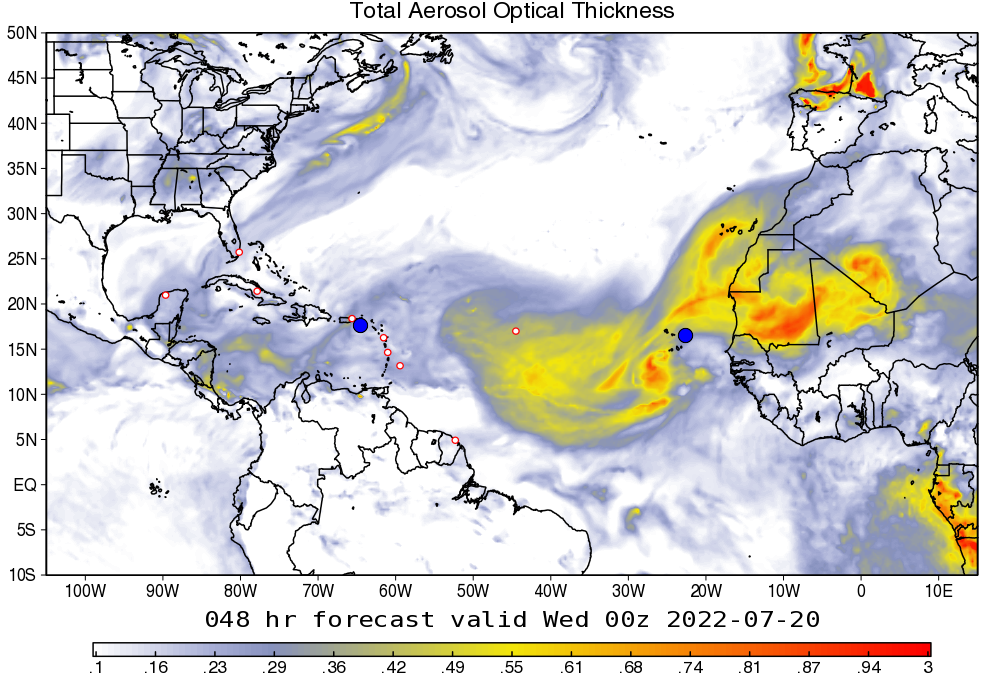
\includegraphics[width=.9\textwidth]{GEOS_total_aot_day2.png}}{
\includegraphics[height=.25\textheight]{logo_cpexcv.png}}}
\end{figure}

\vspace{-.6cm}
\begin{figure}
\textbf{Dust AOT}  \vspace{0.06cm}\\
\begin{tikzpicture}
\node[anchor=south west,inner sep=0] (image) at (0,0) {\frame{\IfFileExists{./figs_cropped/GEOS_dust_aot_day2.png}{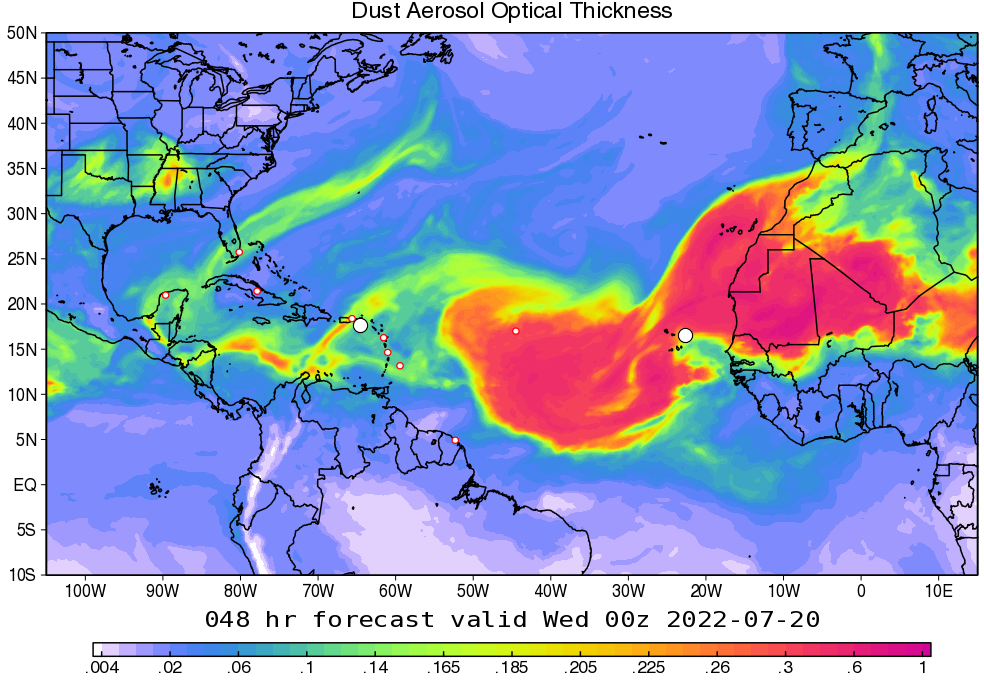
\includegraphics[width=.9\textwidth]{GEOS_dust_aot_day2.png}}{
\includegraphics[height=.25\textheight]{logo_cpexcv.png}}}};
\draw[line width=.2mm, color=black] (1.85,1.) -- (1.85,2.5); %vertical line
\node[text=black] at (1.85, .9) {\tiny 20W};
\draw[line width=.2mm, color=black] (.43,1.6) -- (4., 1.6); %horizontal line
\node[text=black] at (.43, 1.68) {\tiny 15N};
\end{tikzpicture}
\end{figure}
\end{column}


\begin{column}{0.33\textwidth}

\vspace{-0.6cm}
\begin{figure}
\vspace{.1cm}
\textbf{\tiny Cross-section at 15N}  \vspace{0.0cm}\\
\frame{\IfFileExists{./figs_cropped/GEOS_dust_aot_day2_vert_15N.png}{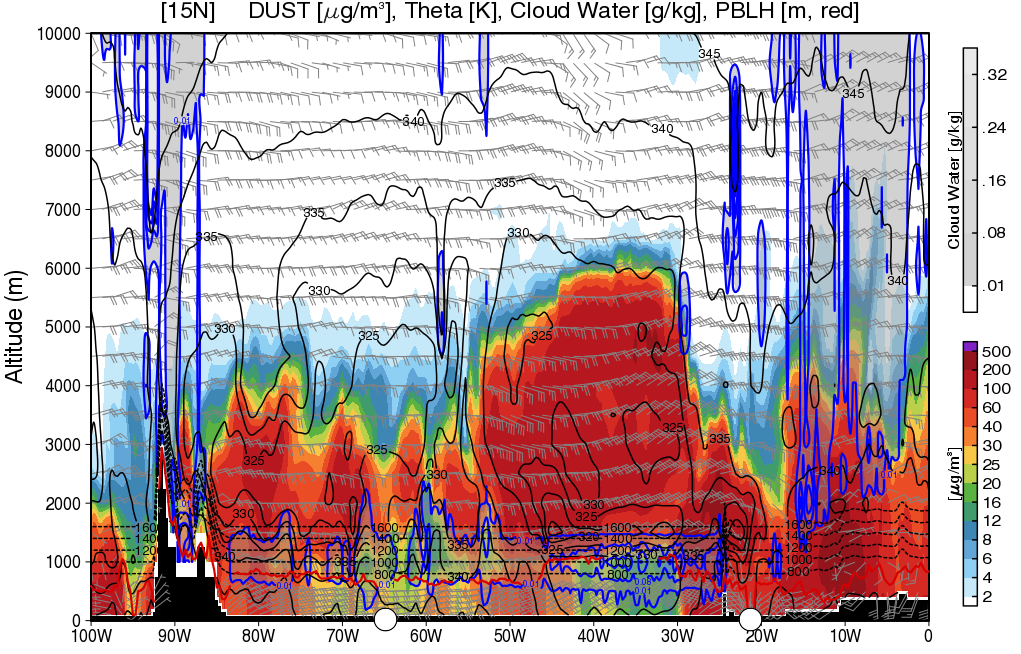
\includegraphics[width=.99\textwidth]{GEOS_dust_aot_day2_vert_15N.png}}{
\includegraphics[height=.25\textheight]{logo_cpexcv.png}}}
\end{figure}


\vspace{-.7cm}
\begin{figure}
\textbf{\tiny Cross-section at 20W}  \vspace{0.0cm}\\
\frame{\IfFileExists{./figs_cropped/GEOS_dust_aot_day2_vert_20W.png}{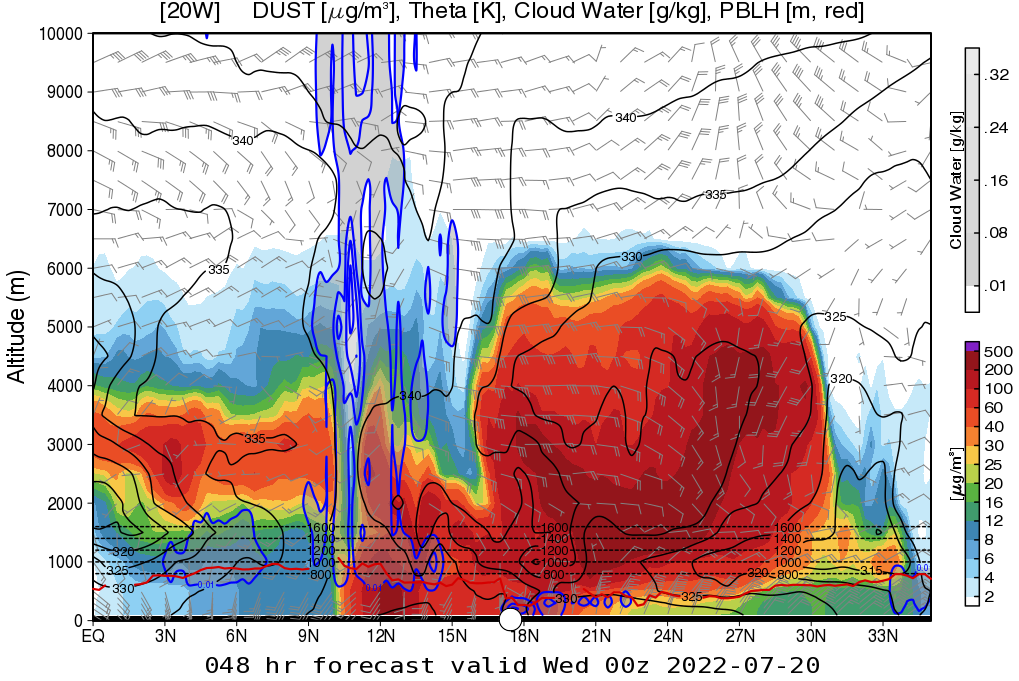
\includegraphics[width=.99\textwidth]{GEOS_dust_aot_day2_vert_20W.png}}{
\includegraphics[height=.25\textheight]{logo_cpexcv.png}}}
\end{figure}

\vspace{2.7cm}


\end{column}

\begin{column}{0.33\textwidth}


\end{column}
\end{columns}

\end{frame}


%%%%%%%%%%%%%%%%%%%%%%%%%%%%%%%%%
%%%%%%%%%%%%%%%%%%%%%%%%%%%%%%%%%
%%%%%%%%%%%%%%%%%%%%%%%%%%%%%%%%%
% % % % % Dust and Aerosol forecast - slide 3
\begin{frame}
\frametitle{Forecast: cloud fraction (days 1 \& 2, {\AdvanceDate[+1]\today}, {\AdvanceDate[+2]\today})}
\vspace{-.4cm}
\begin{center}
\textbf{Day 1}
\end{center}
\vspace{-.75cm}

\begin{columns}
\begin{column}{0.33\textwidth}
\begin{figure}
\textbf{\tiny Low cloud fraction} \\
\frame{\IfFileExists{./figs_cropped/GEOS_lowCloudFraction_day1.png}{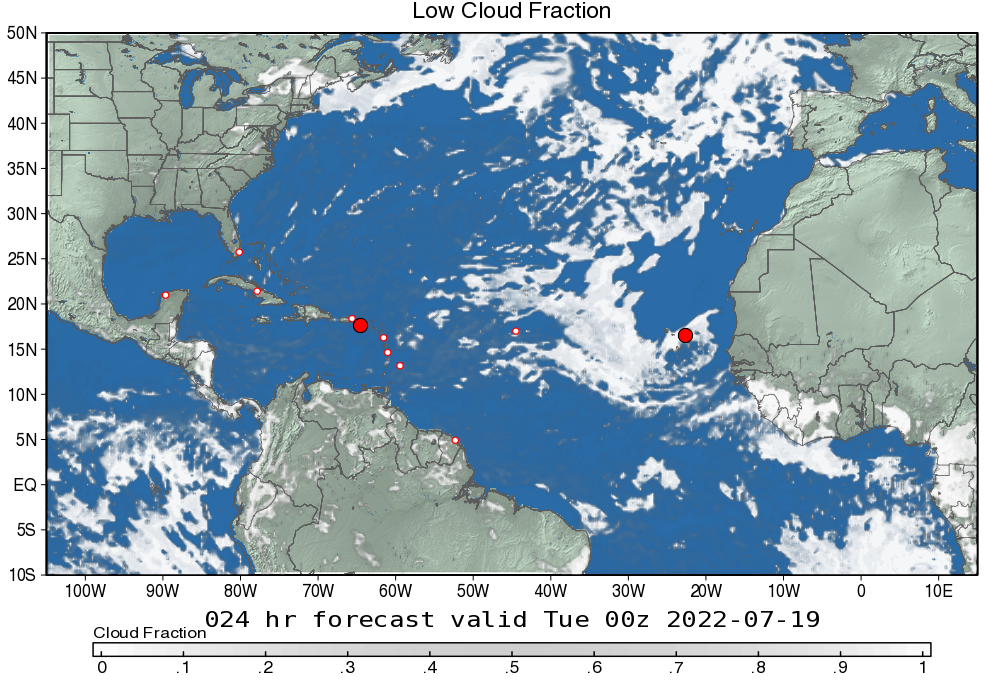
\includegraphics[width=.92\textwidth]{GEOS_lowCloudFraction_day1.png}}{\includegraphics[height=.25\textheight]{logo_cpexcv.png}}}
\end{figure}
\end{column}

\begin{column}{0.33\textwidth}
\begin{figure}
\textbf{\tiny Middle cloud fraction} \\
\frame{\IfFileExists{./figs_cropped/GEOS_midCloudFraction_day1.png}{\includegraphics[width=.92\textwidth]{GEOS_midCloudFraction_day1.png}}{\includegraphics[height=.25\textheight]{logo_cpexcv.png}}}
\end{figure}
\end{column}

\begin{column}{0.33\textwidth}
\begin{figure}
\textbf{\tiny High cloud fraction} \\
\frame{\IfFileExists{./figs_cropped/GEOS_highCloudFraction_day1.png}{\includegraphics[width=.92\textwidth]{GEOS_highCloudFraction_day1.png}}{\includegraphics[height=.25\textheight]{logo_cpexcv.png}}}
\end{figure}
\end{column}
\end{columns}

\vspace{-.1cm}
\begin{center}
\textbf{Day 2}
\end{center}
\vspace{-.5cm}

\begin{columns}
\begin{column}{0.33\textwidth}
\begin{figure}
\frame{\IfFileExists{./figs_cropped/GEOS_lowCloudFraction_day2.png}{\includegraphics[width=.92\textwidth]{GEOS_lowCloudFraction_day2.png}}{\includegraphics[height=.25\textheight]{logo_cpexcv.png}}}
\end{figure}
\end{column}

\begin{column}{0.33\textwidth}
\begin{figure}
\frame{\IfFileExists{./figs_cropped/GEOS_midCloudFraction_day2.png}{\includegraphics[width=.92\textwidth]{GEOS_midCloudFraction_day2.png}}{\includegraphics[height=.25\textheight]{logo_cpexcv.png}}}
\end{figure}
\end{column}

\begin{column}{0.33\textwidth}
\begin{figure}
\frame{\IfFileExists{./figs_cropped/GEOS_highCloudFraction_day2.png}{\includegraphics[width=.92\textwidth]{GEOS_highCloudFraction_day2.png}}{\includegraphics[height=.25\textheight]{logo_cpexcv.png}}}
\end{figure}
\end{column}



\end{columns}


\end{frame}


%%%%%%%%%%%%%%%%%%%%%%%%%%%%%%%%%
%%%%%%%%%%%%%%%%%%%%%%%%%%%%%%%%%
%%%%%%%%%%%%%%%%%%%%%%%%%%%%%%%%%
% % % % % Outlook - slide 1
\begin{frame}
\frametitle{Dust outlook: days 3 \& 4 ({\AdvanceDate[+3]\today}, {\AdvanceDate[+4]\today})}

\vspace{.2cm}

\begin{columns}
\begin{column}{0.5\textwidth}

\vspace{-1.5cm}
\begin{figure}
\textbf{ICAP AOD Ensemble Mean (+3 days)}\vspace{.1cm}\\
\frame{\IfFileExists{./figs_cropped/ICAP_aerosol_ensemble_96.png}{\includegraphics[width=\textwidth]{ICAP_aerosol_ensemble_96.png}}{\includegraphics[height=.25\textheight]{logo_cpexcv.png}}}
\end{figure}

\end{column}
\begin{column}{0.5\textwidth}

\vspace{-1.5cm}
\begin{figure}
\textbf{ICAP AOD Ensemble Mean (+4 days)}\vspace{.1cm}\\
\frame{\IfFileExists{./figs_cropped/ICAP_aerosol_ensemble_120.png}{\includegraphics[width=\textwidth]{ICAP_aerosol_ensemble_120.png}}{\includegraphics[height=.25\textheight]{logo_cpexcv.png}}}
\end{figure}

\end{column}
\end{columns}

\vspace{.1cm}
Comments:


\end{frame}


%%%%%%%%%%%%%%%%%%%%%%%%%%%%%%%%%
%%%%%%%%%%%%%%%%%%%%%%%%%%%%%%%%%
%%%%%%%%%%%%%%%%%%%%%%%%%%%%%%%%%
% % % % % Outlook - slide 2
\begin{frame}
\frametitle{Dynamical outlook: days 3-5 ({\AdvanceDate[+3]\today} - {\AdvanceDate[+5]\today})}


\begin{figure} [htbp]
\begin{center}
\vspace{-0.2cm}
\textbf{700mb Winds and Geopotential Height}

\frame{\IfFileExists{./figs_cropped/GEOS_700mb_outlook_anim_14.png}{\animategraphics[autoplay,loop, height=.8\textheight]{2}{GEOS_700mb_outlook_anim_}{00}{14}}{\includegraphics[height=.25\textheight]{logo_cpexcv.png}}}

\end{center}
\end{figure}


\end{frame}








%%%%%%%%%%%%%%%%%%%%%%%%%%%%%%%%%
%%%%%%%%%%%%%%%%%%%%%%%%%%%%%%%%%
%%%%%%%%%%%%%%%%%%%%%%%%%%%%%%%%%
% % % % % Summary
\begin{frame}
\frametitle{Summary}
\vspace{0cm}
\begin{columns}
\begin{column}{.15\textwidth}
\textbf{Current \\conditions:}

\vspace{1.3cm}
\textbf{Day 1:}

\vspace{1.3cm}
\textbf{Day 2:}

\vspace{1.3cm}
\textbf{Outlook \\(days 3-5):}
\end{column}
\begin{column}{.01\textwidth}

\begin{tikzpicture}
\draw[line width=.2mm, color=black] (0, 0) -- (0, 7);
\end{tikzpicture}



\end{column}
\begin{column}{.83\textwidth}
\end{column}
\end{columns}

\end{frame}





%%%%%%%%%%%%%%%%%%%%%%%%%%%%%%%%%
%%%%%%%%%%%%%%%%%%%%%%%%%%%%%%%%%
%%%%%%%%%%%%%%%%%%%%%%%%%%%%%%%%%
% % % % % Extra slide
%\begin{frame}
%\frametitle{Additional materials}
%
%
%\end{frame}









%%%%%%%%%%%%%%%%%%%%%%%%%%%%%%%%%
%%%%%%%%%%%%%%%%%%%%%%%%%%%%%%%%%
%%%%%%%%%%%%%%%%%%%%%%%%%%%%%%%%%
% % % % % Extra slide
%\begin{frame}
%\frametitle{Additional materials}
%
%
%\end{frame}







\end{document}
